% Shared preamble for the Radioactive Signal Explorer explainers (docs/signals/*.tex).
\documentclass[11pt]{article}
\usepackage[letterpaper,margin=1in]{geometry}
\usepackage[T1]{fontenc}
\usepackage{lmodern}
\usepackage{microtype}
\usepackage{amsmath,amssymb,mathtools,bm}
\usepackage{siunitx}
\usepackage{graphicx}
\usepackage{booktabs,array,tabularx}
\usepackage{xcolor}
\usepackage{enumitem}
\usepackage{caption}
\usepackage[section]{placeins}
\usepackage[most]{tcolorbox}
\usepackage[colorlinks=true,linkcolor=blue!50!black,citecolor=blue!50!black,urlcolor=blue!50!black]{hyperref}
\usepackage[capitalise,noabbrev]{cleveref}
\sisetup{group-separator={,},group-minimum-digits=4,separate-uncertainty}
\definecolor{labblue}{HTML}{0088EE}
\definecolor{exbg}{HTML}{FFF7EC}
\definecolor{boxbg}{HTML}{EEF4FB}
\newtcolorbox{keyidea}[1][]{colback=boxbg,colframe=labblue,boxrule=0.6pt,arc=2pt,left=6pt,right=6pt,top=4pt,bottom=4pt,fonttitle=\bfseries,title={#1}}
\newtcolorbox{pitfall}[1][]{colback=red!3,colframe=red!55!black,boxrule=0.6pt,arc=2pt,left=6pt,right=6pt,top=4pt,bottom=4pt,fonttitle=\bfseries,title={#1}}
\newcounter{exercise}
\newtcolorbox{exercise}[1][]{colback=exbg,colframe=orange!70!black,boxrule=0.6pt,arc=2pt,left=6pt,right=6pt,top=4pt,bottom=4pt,fonttitle=\bfseries,
  title={Exercise~\refstepcounter{exercise}\theexercise\ifx\relax#1\relax\else\ (#1)\fi}}
\newcommand{\dd}{\mathrm{d}}
\newcommand{\keV}{\,\mathrm{keV}}
\newcommand{\MeV}{\,\mathrm{MeV}}
\newcommand{\me}{m_e c^2}
\newcommand{\nuc}[2]{${}^{#1}$#2}
\newcommand{\code}[1]{\texttt{#1}}
\newcommand{\explorer}{\href{https://dark-matter.ucr.edu/Signals.html}{Radioactive Signal Explorer}}
\newcommand{\seriesnote}{\noindent\small This note is one of five explaining the physics behind the \explorer: gamma rays, alpha decay, $(\alpha,n)$ neutrons, beta decay and Cherenkov light. Every figure was computed with the page's own code (\code{assets/signals-physics.js}); the \LaTeX{} sources and figure scripts are in \code{docs/signals/} of \url{https://github.com/UCRDarkMatter/dark-matter-lab-site}. Exercises are marked (A) analytic, (P) programming, (R) open-ended.\normalsize}

\title{The Beta Spectrum, Term by Term:\\ Fermi Function, Corrections, Forbidden Shapes and New Physics}
\author{UCR Dark Matter Lab --- notes for graduate students}
\date{\today}
\begin{document}
\maketitle
\seriesnote

\begin{abstract}
The textbook beta spectrum is phase space times a Fermi function. A spectrum good to $10^{-3}$ or better---what modern searches for neutrino mass, sterile neutrinos and exotic currents need, and what is needed to model low-energy backgrounds in dark-matter detectors---requires about a dozen further factors, each with a clear physical origin. This note follows the review of Hayen \emph{et al.}\ \cite{hayen} and explains every factor implemented in the Beta tab of the Signal Explorer: what it is, how big it is, where it matters, and how it is computed. It then treats forbidden decays and selection rules, and the beyond-Standard-Model (BSM) modifications the tab offers: a neutrino mass, a heavy sterile neutrino and a Fierz interference term.
\end{abstract}
\tableofcontents

\section{Notation and the master formula}
We use natural units with $\hbar = c = \me = 1$, so energies are in units of \SI{511}{keV}. For an electron (or positron) of kinetic energy $T$,
\begin{equation}
W = 1 + \frac{T}{\me}, \qquad p = \sqrt{W^2-1}, \qquad W_0 = 1 + \frac{T_0}{\me}, \qquad q = W_0 - W,
\end{equation}
where $T_0$ is the endpoint and $q$ is the (anti)neutrino energy for a massless neutrino. $Z$ is the charge of the \emph{daughter} nucleus, $A$ its mass number, $R$ its radius (taken as $\sqrt{5/3}$ times the rms charge radius, i.e.\ the radius of the uniform sphere with the same rms), $\alpha$ the fine-structure constant and
\begin{equation}
\gamma_k = \sqrt{k^2 - (\alpha Z)^2}, \qquad \gamma \equiv \gamma_1, \qquad y = \pm\frac{\alpha Z W}{p}\quad(\text{upper sign } \beta^-).
\end{equation}
The spectrum of one branch is
\begin{equation}
\boxed{\;\frac{\dd N}{\dd W} \propto
\underbrace{p\,W\,q^2}_{\text{phase space}}\;
F_0\,L_0\,U\;C\;R\;R_N\,Q\;S\,X\,r\;\times\;\big[\text{forbidden shape}\big]\times\big[\text{BSM}\big]\;}
\label{eq:master}
\end{equation}
and every factor except phase space and $F_0$ is within a few per cent of unity over most of the spectrum. The explorer computes the spectrum on a grid of kinetic energy, multiplies the factors you have switched on, and normalises to unit area (so the CSV is a probability density per keV per decay of that branch). \Cref{tab:terms} summarises them.

\begin{table}[t]
\centering\small
\begin{tabularx}{\linewidth}{@{}l>{\raggedright}X l l@{}}
\toprule
Factor & Physics & Typical size & Hayen eq.\\
\midrule
$F_0$ & Coulomb distortion of the lepton wave function, point nucleus & $\times0.3$--$\times30$ & 6\\
$L_0$ & finite size of a uniformly charged nucleus & \SIrange{0.1}{5}{\%} & 16\\
$U$ & diffuse (realistic) charge distribution & ${\sim}0.1\%$ & 29--30\\
$C$ & lepton wave functions averaged over the nuclear volume; induced currents & \SIrange{0.1}{2}{\%} & 100--106\\
$R$ & radiative corrections (virtual and real photons) & few \% & 48--69\\
$R_N$ & recoil of the nucleus in the phase space & $10^{-5}$--$10^{-3}$ & 41--44\\
$Q$ & recoil of the nuclear Coulomb field & $10^{-5}$--$10^{-3}$ & 45\\
$S$ & screening of the nuclear charge by atomic electrons & up to few \% below \SI{10}{keV} & 144--146\\
$X$ & exchange with atomic electrons ($\beta^-$) & up to tens of \% below few keV & 157\\
$r$ & atomic mismatch (final atom left excited) & near endpoint & 166--167\\
\bottomrule
\end{tabularx}
\caption{Factors in \cref{eq:master}. Equation numbers refer to Hayen \emph{et al.}\ \cite{hayen}.}
\label{tab:terms}
\end{table}

\section{Phase space}
Fermi's golden rule gives a rate proportional to the density of final states. With the nucleus absorbing momentum but (to first approximation) no energy, the electron and neutrino momenta are independent and
\begin{equation}
\dd\Gamma \propto |M|^2\, p^2\,\dd p\; q^2\,\dd q\;\delta(W_0 - W - q)
\;\Longrightarrow\;
\frac{\dd\Gamma}{\dd W} \propto |M|^2\, p W q^2,
\end{equation}
using $p\,\dd p = W\,\dd W$. In the allowed approximation $|M|^2$ is independent of the lepton energies, and this bell shape is the whole spectrum for a neutral daughter.

\section{The Fermi function $F_0$}
The outgoing lepton moves in the Coulomb field of the daughter. Its wave function at the nucleus is enhanced ($\beta^-$, attraction) or suppressed ($\beta^+$, repulsion) relative to a plane wave. Solving the Dirac equation for a point charge and evaluating the lowest partial waves at radius $R$ gives
\begin{equation}
F_0(Z,W) = 4\,(2pR)^{2(\gamma-1)}\,e^{\pi y}\,\frac{|\Gamma(\gamma + iy)|^2}{\Gamma(1+2\gamma)^2}.
\label{eq:F0}
\end{equation}
The radius appears because the point-charge Dirac solution diverges like $r^{\gamma-1}$ at the origin; $F_0$ is defined at the nuclear surface. The non-relativistic limit is the familiar $2\pi y/(1-e^{-2\pi y})$. The code evaluates $\ln|\Gamma(\gamma+iy)|^2$ with a complex Lanczos approximation. \Cref{fig:F0} shows the size of the effect: for $\beta^-$ at high $Z$ the spectrum is enhanced by an order of magnitude at low energy and never goes to zero at $T=0$ (since $F_0 \propto 1/p$ there, cancelling the $p$ of phase space).

\begin{figure}[htbp]
\centering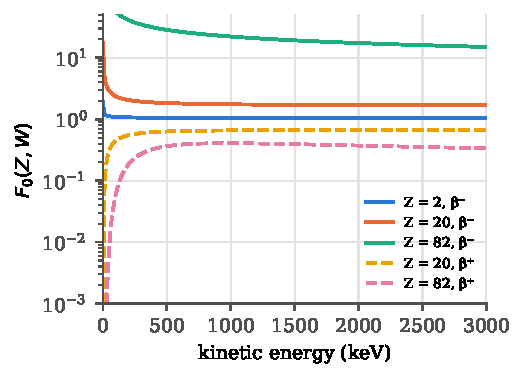
\includegraphics[width=0.62\linewidth]{fig/b_fermi.pdf}
\caption{$F_0$ for $\beta^-$ (solid) and $\beta^+$ (dashed) emission at three daughter charges. Positron emission from heavy nuclei is suppressed by orders of magnitude at low energy.}
\label{fig:F0}
\end{figure}

\begin{pitfall}[Daughter $Z$, and which ``Fermi function''?]
$Z$ is the daughter's charge in both $\beta^-$ and $\beta^+$ decay. Several different quantities are called ``the Fermi function'' in the literature (some include $L_0$, some use $(1+\gamma)/2$ prefactors, some are evaluated at the origin rather than at $R$). Mixing conventions is a common source of percent-level errors at high $Z$.
\end{pitfall}

\section{Finite nuclear size: $L_0$, $U$ and $C$}
\subsection{$L_0$: a uniformly charged sphere}
Inside a finite nucleus the potential is not $-\alpha Z/r$ and the wave functions are less singular. Wilkinson's parametrisation \cite{wilkinson} of the exact solution for a uniformly charged sphere is
\begin{multline}
L_0 = 1 + \frac{13}{60}(\alpha Z)^2 \mp \frac{\alpha Z\,W R\,(41-26\gamma)}{15(2\gamma-1)} \mp \frac{\alpha Z R\,\gamma(17-2\gamma)}{30W(2\gamma-1)}\\
+ a_{-1}\frac{R}{W} + \sum_{n=0}^{5} a_n (WR)^n + 0.41\,(R - 0.0164)(\alpha Z)^{4.5},
\end{multline}
with $a_n = \sum_x b_{x,n}(\alpha Z)^x$ from tabulated coefficients (separately for electrons and positrons; the last constant is 0.22 for $\beta^+$). $L_0$ is between a few tenths of a per cent and several per cent.

\subsection{$U$: a diffuse surface}
Real nuclei have a Fermi-shaped charge distribution with a skin. Wilkinson's correction relative to the uniform sphere is
\begin{equation}
U = 1 + a_0 + a_1 p + a_2 p^2, \qquad a_i = a_i(Z, \text{sign}),
\end{equation}
about $10^{-3}$.

\subsection{$C$: the convolution with the nuclear volume and induced currents}
The decay happens throughout the nucleus, not at its centre, so the product of lepton wave functions must be averaged over the nuclear volume weighted by the transition density. For an allowed decay this gives
\begin{equation}
C(W) = 1 + C_0 + C_1 W + \frac{C_{-1}}{W} + C_2 W^2,
\end{equation}
separately for the vector (Fermi) and axial (Gamow--Teller) parts, combined with the mixing ratio
\begin{equation}
\rho = \frac{C_A M_\text{GT}}{C_V M_F}, \qquad C = \frac{C_V^{\text{(shape)}} + \rho^2\, C_A^{\text{(shape)}}}{1 + \rho^2}.
\end{equation}
$\rho = 0$ is a pure Fermi decay ($0^+\to0^+$), $\rho\to\infty$ pure Gamow--Teller. The vector coefficients are
\begin{align}
C_0^V &= -\tfrac{233}{630}(\alpha Z)^2 - \tfrac15 (W_0R)^2 \mp \tfrac{6}{35}\alpha Z W_0 R, &
C_1^V &= \mp\tfrac{13}{35}\alpha Z R + \tfrac{4}{15}W_0R^2,\nonumber\\
C_{-1}^V &= \tfrac{2}{15}W_0R^2 \pm \tfrac{1}{70}\alpha Z R, &
C_2^V &= -\tfrac{4}{15}R^2 .
\end{align}
The axial coefficients contain, in addition, the \emph{induced currents}, which appear because the nucleons are composite and the hadronic current has more structure than $\gamma^\mu(1-\gamma_5)$:
\begin{itemize}
\item \textbf{Weak magnetism} $b/Ac$: the weak analogue of the isovector magnetic moment, fixed by the conserved vector current (CVC) hypothesis, $b/Ac \approx \mu_p - \mu_n \approx 4.7$ in the impulse approximation. Its leading effect is a linear slope $C \supset \pm\frac{4}{3}\frac{b}{Ac}\frac{W}{M_N}$, about $\pm0.5\%$ per MeV. It is Standard Model physics, but it mimics a Fierz term and is one of the main systematics in BSM searches with Gamow--Teller decays. The Beta tab lets you switch it separately.
\item \textbf{Induced tensor} $d/Ac$: a ``second-class current'', zero in the Standard Model for mirror decays by $G$-parity.
\item $\Lambda = M_{1y}/M_{1}$-type ratio of nuclear matrix elements, which enters the $R^2$ terms; set to zero unless you have a shell-model value.
\end{itemize}
The induced pseudoscalar term is suppressed by $m_e/M_N$ squared and omitted. The full expressions are Hayen eqs.\ 105--106 and are written out in the generated code.

\section{Radiative corrections $R$}
Photons exchanged between the charged particles, and real photons emitted in the decay (inner bremsstrahlung), modify the spectrum. The infrared divergences of the two cancel, leaving a finite, energy-dependent correction:
\begin{equation}
R = 1 + \delta_1 + \delta_2 + \delta_3 + \cdots
\end{equation}
\begin{description}[leftmargin=1.2em]
\item[Order $\alpha$ (Sirlin)] $\delta_1 = \frac{\alpha}{2\pi}\left[g(W_0,W) - 3\ln\frac{M_p}{2W_0}\right]$, with Sirlin's universal function
\begin{multline}
g = 3\ln M_p - \tfrac34 - \frac{4}{\beta}\,\mathrm{Li}_2\!\left(\frac{2\beta}{1+\beta}\right) + 4\left(\frac{\tanh^{-1}\beta}{\beta} - 1\right)\left[\frac{W_0-W}{3W} - \frac32 + \ln\big(2(W_0-W)\big)\right]\\
+ \frac{\tanh^{-1}\beta}{\beta}\left[2(1+\beta^2) + \frac{(W_0-W)^2}{6W^2} - 4\tanh^{-1}\beta\right],
\end{multline}
$\beta = p/W$ and $M_p$ the proton mass (Hayen eq.\ 50 writes the dilogarithm term with Spence's function $L(x) = -\mathrm{Li}_2(x)$). The $\ln(W_0 - W)$ term diverges at the endpoint, where soft photons cannot be treated perturbatively.
\item[Endpoint resummation (Repko--Wu)] Summing soft-photon emission to all orders replaces the logarithm by a power, $1 + \frac{2\alpha}{\pi}(\frac{\tanh^{-1}\beta}{\beta}-1)\ln(W_0-W) \to (W_0-W)^{t}$ with $t = \frac{2\alpha}{\pi}\left(\frac{\tanh^{-1}\beta}{\beta}-1\right)$, which goes smoothly to zero at the endpoint.
\item[Order $Z\alpha^2$ and $Z^2\alpha^3$] Nucleus-dependent corrections (Sirlin; Jaus; Wilkinson) that depend on $Z$, on the nuclear size through the cut-off $\Lambda = \sqrt6/r_\text{rms}$, and on the nucleon form factors. They are switchable separately (``higher-order radiative'').
\end{description}
The energy-independent part of the radiative correction (the short-distance enhancement $\approx1.02$) does not change the spectral shape; the code divides it out so that $R\approx1$ in the middle of the spectrum. \Cref{fig:fac} shows $R$ as a few-per-cent tilt that grows towards the endpoint.

\section{Recoil corrections $R_N$ and $Q$}
The daughter is not infinitely heavy. Including its recoil in the three-body phase space and in the hadronic current gives $R_N = 1 + r_0 + r_1/W + r_2 W + r_3/W^2$ with coefficients of order $W_0/M$ and $W_0^2/M^2$, different for vector and axial parts (weighted with $\rho$ like $C$). The recoiling nucleus also carries its Coulomb field away from the leptons:
\begin{equation}
Q = 1 \mp \frac{\pi\alpha Z}{M p}\left(1 + a\,\frac{W_0-W}{3W}\right), \qquad a = \frac{1-\rho^2/3}{1+\rho^2}.
\end{equation}
Both are $10^{-5}$--$10^{-3}$. They matter for precision $\beta$--$\nu$ correlation work and, together, for the light nuclei (tritium, \nuc{6}{He}) where $M$ is smallest.

\section{Atomic effects: $S$, $X$ and $r$}
\subsection{Screening $S$}
Far from the nucleus the atomic electrons screen its charge, so the lepton feels a weaker potential than $-\alpha Z/r$. Rose's prescription, refined by Bühring, describes the screened potential by a constant shift $V_0$ in the lepton's energy at large distances:
\begin{gather}
S = \frac{\tilde W}{W}\;
\frac{|\Gamma(\gamma + i\tilde y)|^2}{|\Gamma(\gamma + iy)|^2}\;
\frac{|\Gamma(\gamma + 2i\tilde p/\lambda)|^2}{|\Gamma(1 + 2ip/\lambda)|^2}\;
e^{-\pi y}\left(\frac{2p}{\lambda}\right)^{2(1-\gamma)},\\
\tilde W = W \mp V_0,\quad \tilde p = \tfrac12 p + \tfrac12\sqrt{p^2 \mp 2\alpha Z\tilde W\lambda},\quad
\tilde y = \pm\frac{\alpha Z\tilde W}{\tilde p},\quad \lambda = \frac{2V_0}{\alpha Z},\quad V_0 = 1.45\,\alpha^2 Z_\text{parent}^{4/3},\nonumber
\end{gather}
(Hayen eqs.\ 144--146, with the coefficient $N = 1.45$ in $V_0$), where $V_0$ is the potential energy shift due to the electron cloud and $\lambda$ the inverse screening length. Screening lowers $\beta^-$ and raises $\beta^+$ spectra at low energy: about 1\% at \SI{10}{keV} for medium $Z$. The prescription is undefined for $W - 1 \lesssim V_0$ (a few hundred eV for heavy atoms); below that the code continues it at its value at the edge of validity rather than letting it jump.

\subsection{Exchange $X$}
In $\beta^-$ decay the electron can be created directly in an empty bound orbital of the daughter while an atomic electron is ejected into the same continuum state. The two final states are indistinguishable, so their amplitudes interfere. The effect is large at low energy: tens of per cent below a few keV for \nuc{63}{Ni}, \nuc{241}{Pu} and tritium (\cref{fig:fac}). Hayen \emph{et al.}\ fit Nitescu-type calculations with
\begin{equation}
X = 1 + \frac{a}{W'} + \frac{b}{W'^2} + c\,e^{-dW'} + e\,\frac{\sin\left[(W - f)^g + h\right]}{W^i}, \qquad W' = W - 1,
\end{equation}
with nine coefficients per $Z$ (their Table X, $Z = 2$--$100$, in \code{assets/signals-exchange.js}). There is no exchange correction for $\beta^+$.

\subsection{Mismatch $r$}
The parent atom's electron cloud is not an eigenstate of the daughter atom, so the daughter is usually left excited (shake-up, shake-off). On average this costs
\begin{equation}
\Delta E = \frac12\,\frac{\partial^2 B}{\partial Z^2}, \qquad \frac{\partial^2 B}{\partial Z^2} \approx 44.200\,Z^{0.41} + 2.3196\times10^{-7}\,Z^{4.45}\ \text{eV},
\end{equation}
where $B(Z)$ is the total electron binding energy of the atom and the fit is Hayen eq.\ 167 ($\Delta E \approx \SI{29}{eV}$ for a helium daughter, \SI{88}{eV} for copper). Hayen's $r = 1 - \frac{2\Delta E}{W_0 - W}$ is the first-order expansion of shifting the endpoint by $\Delta E$ in $q^2$. The explorer uses the shift itself,
\begin{equation}
r = \left(\frac{W_0 - W - \Delta E}{W_0 - W}\right)^2 \quad (W_0 - W > \Delta E), \qquad 0 \text{ otherwise},
\end{equation}
which agrees with Hayen's form away from the endpoint and, unlike it, ends the spectrum smoothly instead of producing a negative region. Neither form describes the discrete structure of the real final-state spectrum (for tritium the \nuc{3}{He}$^+$ ground state takes about 57\% and the rest is spread over tens of eV); for neutrino-mass work the final-state distribution must be convolved explicitly, and the BSM endpoint figure below switches $r$ off for that reason.

\begin{figure}[htbp]
\centering
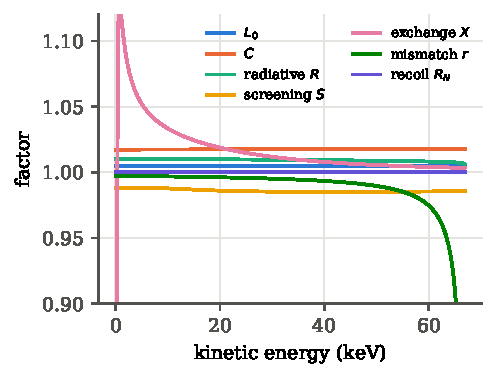
\includegraphics[width=0.49\linewidth]{fig/b_fac63.pdf}\hfill
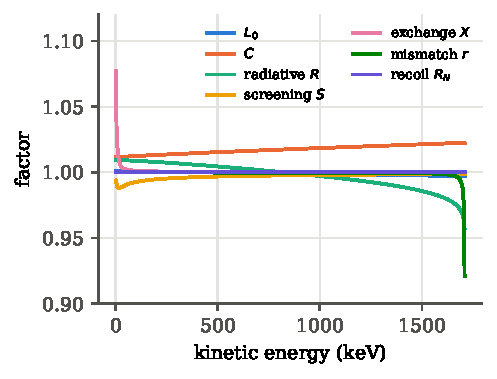
\includegraphics[width=0.49\linewidth]{fig/b_fac32.pdf}
\caption{Every correction factor except $F_0$ for \nuc{63}{Ni} ($T_0 = \SI{67}{keV}$, left) and \nuc{32}{P} ($T_0 = \SI{1711}{keV}$, right). For the low-energy emitter the atomic effects (exchange, screening) dominate; for the high-energy one, radiative corrections and finite size do. The exchange spike at the lowest energies of \nuc{63}{Ni} is cut off by the axis.}
\label{fig:fac}
\end{figure}

\section{Forbidden decays}
\subsection{Selection rules}
In the allowed approximation the leptons carry no orbital angular momentum. The Fermi operator (vector, $\mathbb{1}$) then requires $\Delta J = 0$ and the Gamow--Teller operator (axial, $\bm\sigma$) $\Delta J = 0,1$ (not $0\to0$), both without parity change. When these are forbidden by the spins and parities, the leptons must carry orbital angular momentum $L = k$, each unit costing a factor of order $(pR)^2$ or $(qR)^2 \sim 10^{-3}$--$10^{-4}$ in rate:
\begin{center}\small
\begin{tabular}{@{}lll@{}}
\toprule
Type & $\Delta J$ & $\pi_i\pi_f$ \\
\midrule
allowed (superallowed if $0^+\to0^+$ or mirror) & $0, 1$ & $+$\\
first forbidden non-unique & $0, 1$ & $-$ \\
first forbidden unique & $2$ & $-$\\
second forbidden non-unique & $2$ & $+$ \\
second forbidden unique & $3$ & $+$\\
$k$-th forbidden unique & $k+1$ & $(-1)^k$\\
\bottomrule
\end{tabular}
\end{center}
The tab takes the transition type from ENSDF when the evaluation gives one; otherwise it derives it from the parent and daughter-level $J^\pi$ (looked up from the level schemes) with these rules, flagging tentative assignments.

\subsection{Unique forbidden shapes}
For a unique $k$-th forbidden transition a single nuclear matrix element contributes, so the shape is fixed by the lepton wave functions alone:
\begin{equation}
C_k(W) \propto \sum_{n=1}^{k+1} \lambda_n\,
\frac{p^{2(n-1)}\,q^{2(k+1-n)}}{(2n-1)!\,\big[2(k+1-n)+1\big]!},
\qquad
\lambda_n = \frac{F_{n-1}}{F_0}\,\frac{n + \gamma_n}{n(1+\gamma_1)},
\label{eq:unique}
\end{equation}
where $F_{n-1}$ is the generalised Fermi function for the $n$-th partial wave,
\begin{equation}
F_{k-1} = \left[k\,(2k-1)!!\right]^2 4^k\,(2pR)^{2(\gamma_k-k)}\,e^{\pi y}\,\frac{|\Gamma(\gamma_k+iy)|^2}{\Gamma(1+2\gamma_k)^2}.
\end{equation}
Without Coulomb effects $\lambda_n = 1$; with them the higher partial waves of the electron are enhanced for $\beta^-$. For first-forbidden unique decays ($k=1$) the shape is $\propto q^2 + \lambda_2 p^2$, which hardens the spectrum. \Cref{fig:unique} compares the unique and allowed shapes for \nuc{90}{Y} and \nuc{40}{K}.

\begin{figure}[htbp]
\centering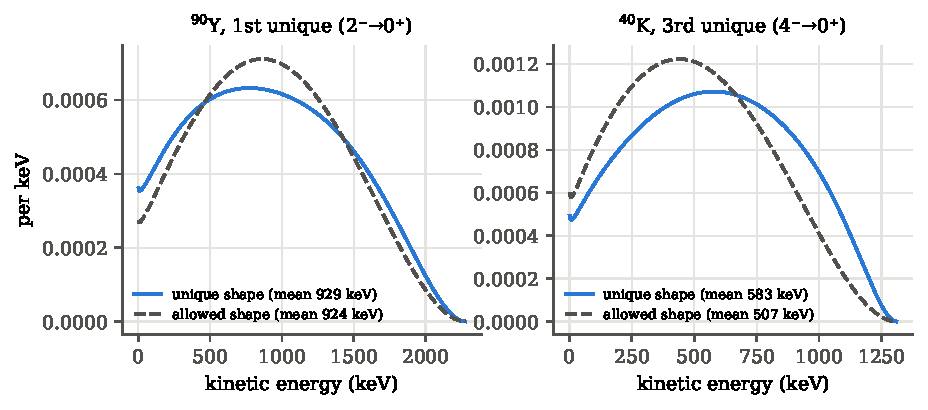
\includegraphics[width=\linewidth]{fig/b_unique.pdf}
\caption{Unique-forbidden shapes (\cref{eq:unique}) versus the allowed shape for \nuc{90}{Y} (first forbidden unique, $2^-\to0^+$; means 929 vs \SI{924}{keV}) and \nuc{40}{K} (third forbidden unique, $4^-\to0^+$; means 583 vs \SI{507}{keV}). The ENSDF mean for \nuc{40}{K} is \SI{560}{keV}: measured \nuc{40}{K} spectra deviate from the theoretical unique shape, which is a known open problem.}
\label{fig:unique}
\end{figure}

\subsection{Non-unique forbidden decays}
Here several nuclear matrix elements contribute with energy-dependent lepton factors, and they can interfere. When one combination dominates and the Coulomb energy $\alpha Z/2R$ is large compared with $W_0$ (the ``$\xi$ approximation''), the shape is close to allowed, which is the default. Otherwise the shape must come from a nuclear-structure calculation or a measurement; the tab accepts an empirical shape factor $1 + aW + b/W + cW^2$ for this (and for any other case where you want to override the theory).

\section{Beyond the Standard Model}
\subsection{Neutrino mass}
With a neutrino mass $m_\nu$ the neutrino phase space becomes $q\sqrt{q^2 - m_\nu^2}$ instead of $q^2$, and the spectrum ends $m_\nu$ below the massless endpoint. Because the neutrino is a superposition of mass eigenstates, what is measured is
\begin{equation}
\frac{\dd N}{\dd W} \propto \sum_i |U_{ei}|^2\,q\sqrt{q^2 - m_i^2}\;\Theta(q - m_i) \;\approx\; q\sqrt{q^2 - m_\beta^2}, \qquad m_\beta^2 = \sum_i |U_{ei}|^2 m_i^2,
\end{equation}
when the $m_i$ are not resolved. The effect lives in the last few eV (\cref{fig:tritium}), which is why tritium (\SI{18.6}{keV} endpoint, superallowed, simple atomic structure) is the isotope of choice; KATRIN currently limits $m_\beta < \SI{0.45}{eV}$ (90\% CL) \cite{katrin}.

\begin{figure}[htbp]
\centering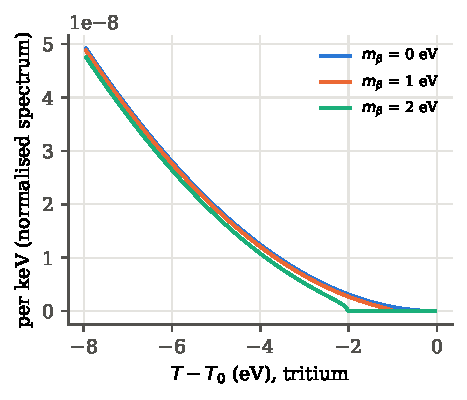
\includegraphics[width=0.6\linewidth]{fig/b_tritium.pdf}
\caption{The last \SI{8}{eV} of the tritium spectrum (all corrections except the mismatch $r$, which shifts the endpoint by \SI{29}{eV} on average and would need a proper final-state distribution here) for $m_\beta = 0$, 1 and \SI{2}{eV}. Only a fraction $\sim10^{-13}$ of decays fall in the last eV.}
\label{fig:tritium}
\end{figure}

\subsection{A heavy (sterile) neutrino}
If the electron neutrino has a small admixture $|U_{e4}|^2$ of a heavy state of mass $m_4$ (keV-scale sterile neutrinos are warm-dark-matter candidates), the spectrum is the incoherent sum
\begin{equation}
\frac{\dd N}{\dd W} = (1 - |U_{e4}|^2)\,N(W; m_\beta) + |U_{e4}|^2\,N(W; m_4),
\end{equation}
with both branches computed with all the same corrections. The heavy branch stops at $T_0 - m_4$, producing a kink there (\cref{fig:bsm}). In the tab this is a separate switch, with $m_4$ in keV and $|U_{e4}|^2$ as a mixing probability, independent of the light-neutrino mass $m_\beta$ (in eV). Laboratory searches (e.g.\ TRISTAN at KATRIN) aim at $|U_{e4}|^2 \sim 10^{-6}$--$10^{-8}$, which requires understanding every factor in \cref{eq:master} to that level.

\subsection{The Fierz term}
In the most general Lorentz-invariant contact interaction, the Standard Model's vector and axial couplings $C_V$, $C_A$ are joined by scalar and tensor couplings $C_S, C_S', C_T, C_T'$. To first order in the exotic couplings, their interference with the Standard Model adds a term to the spectrum \cite{jtw}:
\begin{equation}
\frac{\dd N}{\dd W} \to \frac{\dd N}{\dd W}\left(1 + b_F\,\frac{\gamma}{W}\right),\qquad
b_F = \pm\frac{1}{1+\rho^2}\left[\mathrm{Re}\frac{C_S + C_S'}{C_V} + \rho^2\,\mathrm{Re}\frac{C_T + C_T'}{C_A}\right],
\label{eq:fierz}
\end{equation}
upper sign for $\beta^-$ (here $\gamma = \gamma_1$; many papers write $m_e/E_e$, the $\alpha Z\to0$ limit). Pure Fermi decays probe scalar couplings and pure Gamow--Teller decays tensor couplings; mixed decays probe both. Current limits are $|b_F| \lesssim$ a few $\times10^{-3}$ from superallowed $0^+\to0^+$ decays and $\sim10^{-2}$ from Gamow--Teller spectra.

The tab offers one Fierz control with three modes, so that $b_F$ is never specified twice: off; enter $b_F$ directly; or enter the two coupling combinations in \cref{eq:fierz} and let the page compute $b_F$ with the branch's $\rho$ and sign (the computed value is displayed). Because $\gamma/W$ is largest at low energy, the Fierz term tilts the spectrum towards low energies for $b_F>0$; note that the overall normalisation absorbs part of it, so the measurable effect is a \emph{shape} distortion (\cref{fig:bsm}), and that weak magnetism produces a similar tilt.

\begin{figure}[htbp]
\centering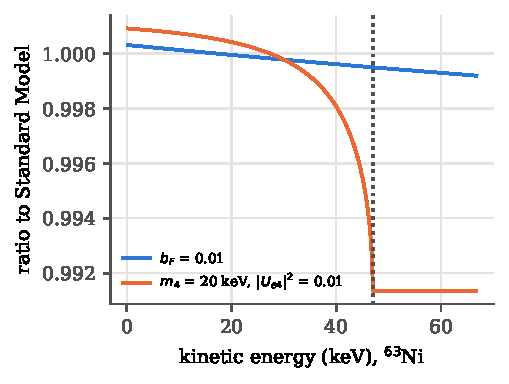
\includegraphics[width=0.6\linewidth]{fig/b_bsm.pdf}
\caption{Ratio to the Standard Model spectrum of \nuc{63}{Ni} for a Fierz term $b_F = 0.01$ and for a \SI{20}{keV} sterile neutrino with $|U_{e4}|^2 = 0.01$. The dotted line marks $T_0 - m_4$.}
\label{fig:bsm}
\end{figure}

\section{What the Beta tab outputs, and checks}
For an isotope the tab lists every $\beta^\pm$ branch with endpoint, intensity, daughter level and transition type, and computes the intensity-weighted sum; for a custom decay you give $Z$, $A$, $T_0$, the type and $\rho$. Every factor of \cref{eq:master} has its own switch, and the plot can show the factors themselves. The outputs are a CSV, the formula with the numerical values of the constants used, and standalone Python and C++ programs implementing exactly the selected terms (they reproduce the page to a few parts in $10^6$).

As checks, the mean energies with all corrections agree with ENSDF to 0.2\% or better: \nuc{3}{H} 5.69 (ENSDF 5.69), \nuc{14}{C} 49.11 (49.16), \nuc{32}{P} 693.7 (695.0), \nuc{22}{Na} 215.2 (215.5) and \nuc{90}{Y} \SI{927.0}{keV} (926.7). For \nuc{63}{Ni} the page gives \SI{17.32}{keV} against ENSDF's \SI{17.43}{keV}; the difference is the exchange correction, which the ENSDF/LogFT mean does not include.

\section{Exercises}
\begin{exercise}[A]
Show that $F_0$ in \cref{eq:F0} reduces to $2\pi y/(1-e^{-2\pi y})$ when $\alpha Z\to0$ at fixed $y$. Then show that for $\beta^-$ the product $pWq^2F_0$ tends to a non-zero constant at $p\to0$.
\end{exercise}
\begin{exercise}[A]
The Kurie plot $K(W) = \sqrt{\frac{\dd N/\dd W}{pWF}}$ is linear in $W$ for an allowed decay with a massless neutrino. Show how a neutrino mass and a unique first-forbidden shape each bend it, and why this made the Kurie plot the standard tool for endpoint measurements.
\end{exercise}
\begin{exercise}[A]
Show that for small $b_F$ the change in the mean energy is $\delta\langle T\rangle \approx b_F\,\gamma\left[\langle T/W\rangle - \langle T\rangle\langle 1/W\rangle\right]$ (in $\me$ units). Using the explorer, estimate the precision on $\langle T\rangle$ needed for \nuc{6}{He} to reach $|b_F| = 10^{-3}$, and compare with the weak-magnetism slope.
\end{exercise}
\begin{exercise}[P]
Write the allowed spectrum with $F_0$ only, then add $L_0$, $C$, $R$, $S$, $X$ one at a time for \nuc{63}{Ni}, and plot each new spectrum's ratio to the previous one. Compare with the Python program the tab generates.
\end{exercise}
\begin{exercise}[P]
Fit the tritium endpoint region simulated by the explorer (all corrections, $m_\beta = 0$) with a pure phase-space model $q\sqrt{q^2-m^2}$ times a constant, floating $m^2$ and $T_0$. What bias do you get in $m^2$ if you fit the last 40 eV, and why? (This is why KATRIN's model includes everything in \cref{eq:master} and the final-state distribution.)
\end{exercise}
\begin{exercise}[R]
\nuc{39}{Ar} ($7/2^-\to3/2^+$, $T_0 = \SI{565}{keV}$) is the dominant background in argon dark-matter detectors. Classify the transition, explain which spectral shape you would use, and discuss which of the corrections in \cref{tab:terms} matter for the background in the \SIrange{0}{100}{keV} region.
\end{exercise}

\begin{thebibliography}{9}
\bibitem{hayen} L.~Hayen, N.~Severijns, K.~Bodek, D.~Rozpedzik and X.~Mougeot, ``High precision analytical description of the allowed $\beta$ spectrum shape'', Rev.\ Mod.\ Phys.\ \textbf{90}, 015008 (2018), arXiv:1709.07530.
\bibitem{wilkinson} D.~H. Wilkinson, ``Evaluation of beta-decay I. The traditional phase space factors'', Nucl.\ Instrum.\ Meth.\ A \textbf{275}, 378 (1989); ``\ldots II. Finite mass and size effects'', \textbf{290}, 509 (1990).
\bibitem{behrens} H.~Behrens and W.~B\"uhring, \emph{Electron Radial Wave Functions and Nuclear Beta-Decay} (Clarendon, Oxford, 1982).
\bibitem{sirlin} A.~Sirlin, ``General properties of the electromagnetic corrections to the beta decay of a physical nucleon'', Phys.\ Rev.\ \textbf{164}, 1767 (1967); W.~W. Repko and C.-E. Wu, Phys.\ Rev.\ C \textbf{28}, 2433 (1983).
\bibitem{jtw} J.~D. Jackson, S.~B. Treiman and H.~W. Wyld, ``Possible tests of time reversal invariance in beta decay'', Phys.\ Rev.\ \textbf{106}, 517 (1957).
\bibitem{gonzalez} M.~Gonz\'alez-Alonso, O.~Naviliat-Cuncic and N.~Severijns, ``New physics searches in nuclear and neutron $\beta$ decay'', Prog.\ Part.\ Nucl.\ Phys.\ \textbf{104}, 165 (2019).
\bibitem{katrin} KATRIN Collaboration, ``Direct neutrino-mass measurement based on 259 days of KATRIN data'', Science \textbf{388}, 180 (2025).
\end{thebibliography}
\end{document}
